\documentclass[12pt,titlepage,a4paper]{article}

\pagestyle{headings}
\usepackage{hyperref}
\usepackage[utf8]{inputenc}
\usepackage{amssymb,amsmath,amsthm}
\usepackage{systeme,mathtools}
\usepackage{indentfirst}
\usepackage{circuitikz}
\usepackage{tikz}
\setlength{\parindent}{3ex}
%%%%%%%%%%%%%%%%%%%%%%%%%%%%%%%%%%%%%%%%%%%%%%%%%%%%%%%%%%%%%%%%%%%%%%%%%%%%%%%%%%%%%%%%%%%%%
%%%%%%%%%%%%%%%%%%                Realizator: Pop Adrian              %%%%%%%%%%%%%%%%%%%%%%%
%%%%%%%%%%%%%%%%%%%%%%%%%%%%%%%%%%%%%%%%%%%%%%%%%%%%%%%%%%%%%%%%%%%%%%%%%%%%%%%%%%%%%%%%%%%%%
\usetikzlibrary{backgrounds}
\makeatletter

%% \pgf@circ@Rlen = \pgfkeysvalueof{/tikz/circuitikz/bipoles/length}
%% Commenting the line above apparently solved the missing "Missing number, treated as zero" error

\def\TikzBipolePath#1#2{\pgf@circ@bipole@path{#1}{#2}}
\makeatother

\newlength{\ResUp} 
\newlength{\ResRight}

%%%%%%%%%%%%%%%%%%%%%%%%%%%%%%%%%%%%%%%%%%%%%%%%%%%%%%%%%%%%%%%%%%%%%%%%%%%%%%%%%%%%%%%%%%%%%
%%%%%%%%%%%%%%%%%%      Sursa de curent: simbol folosit in Romania    %%%%%%%%%%%%%%%%%%%%%%%
%%%%%%%%%%%%%%%%%%%%%%%%%%%%%%%%%%%%%%%%%%%%%%%%%%%%%%%%%%%%%%%%%%%%%%%%%%%%%%%%%%%%%%%%%%%%%
%Declaram dimensiunile initiale
\ctikzset{bipoles/romanianCurrentSource/height/.initial=.60}
\ctikzset{bipoles/romanianCurrentSource/width/.initial=.60}

%Definim noul simbol pentru SIC
\pgfcircdeclarebipole{} 
	%Offset pentru label-uri
	{\ctikzvalof{bipoles/romanianCurrentSource/height}}
	%Numele simbolului
	{romanianCurrentSource}
	%Dimensiunile "cutiei" in care va sta
	{\ctikzvalof{bipoles/romanianCurrentSource/height}}
	{\ctikzvalof{bipoles/romanianCurrentSource/width}}
	{
		%Stabilim grosimea standard a liniei pentru un element
		\pgfsetlinewidth{\pgfkeysvalueof{/tikz/circuitikz/bipoles/thickness}\pgfstartlinewidth}
		
		%Definim ancorele
		\pgfextracty{\ResUp}{\northeast}
		\pgfextractx{\ResRight}{\southwest}
		
		%Desenam cerculetul
		\pgfpathellipse{\pgfpointorigin}{\pgfpoint{0cm}{\ResUp}}{\pgfpoint{\ResRight}{0cm}}
		
		%Desenam prima sagetica; trebuie sa avem grija ca dupa ce desenam un segment,
		%urmatoarea linie va fi desenata relativ la capatul segmentului, nu fata de
		%origine, deci sunt necesare cateva repozitionari
		\pgfmoveto{\pgfpoint{1.0\ResRight}{0.0\ResUp}}   %Ne pozitionam in (-1, 0)
		\pgflineto{\pgfpoint{0.1\ResRight}{0.0\ResUp}}   %Desenam corpul sagetii
		\pgflineto{\pgfpoint{0.3\ResRight}{-0.25\ResUp}} %Desenam unul din capete
		\pgfmoveto{\pgfpoint{0.1\ResRight}{0.0\ResUp}}   %Ne pozitionam in (-0.1, 0)
	    \pgflineto{\pgfpoint{0.3\ResRight}{0.25\ResUp}}  %Desenam celalalt capat
		
		%Desenam ce-a de-a doua sagetica
		\pgfmoveto{\pgfpoint{-0.2\ResRight}{0.0\ResUp}}  %Ne pozitionam in (0.2, 0)
		\pgflineto{\pgfpoint{-1.0\ResRight}{0.0\ResUp}}  %Desenam corpul sagetii
		\pgfmoveto{\pgfpoint{0.0\ResRight}{0.25\ResUp}}  %Ne repozitionam
		\pgflineto{\pgfpoint{-0.2\ResRight}{0.0\ResUp}}  %Desenam unul din capete
		\pgflineto{\pgfpoint{0.0\ResRight}{-0.25\ResUp}} %Desenam celalat capat
		
		%Pentru desenare, sa folosim functia draw
		\pgfusepath{draw}
	}

%Ii definim un stil si o cale si...gata!
\def\romanianCurrentSourcepath#1{\TikzBipolePath{romanianCurrentSource}{#1}}
\tikzset{romanianCurrentSource/.style = {\circuitikzbasekey, /tikz/to path=\romanianCurrentSourcepath, l=#1}}


%%%%%%%%%%%%%%%%%%%%%%%%%%%%%%%%%%%%%%%%%%%%%%%%%%%%%%%%%%%%%%%%%%%%%%%%%%%%%%%%%%%%%%%%%%%%%
%%%%%%%%%%%%%%%%%%      Sursa de tensiune: simbol folosit in Romania    %%%%%%%%%%%%%%%%%%%%
%%%%%%%%%%%%%%%%%%%%%%%%%%%%%%%%%%%%%%%%%%%%%%%%%%%%%%%%%%%%%%%%%%%%%%%%%%%%%%%%%%%%%%%%%%%%%
%Declaram dimensiunile initiale
\ctikzset{bipoles/romanianVoltageSource/height/.initial=.60}
\ctikzset{bipoles/romanianVoltageSource/width/.initial=.60}

%Definim noul simbol pentru SIT
\pgfcircdeclarebipole{}
	%Stabilim grosimea standard a liniei pentru un element
	{\ctikzvalof{bipoles/romanianVoltageSource/height}}
	%Numele simbolului
	{romanianVoltageSource}
	%Dimensiunile "cutiei" in care va sta
	{\ctikzvalof{bipoles/romanianVoltageSource/height}}
	{\ctikzvalof{bipoles/romanianVoltageSource/width}}
	{
		%Stabilim grosimea standard a liniei pentru un element
		\pgfsetlinewidth{\pgfkeysvalueof{/tikz/circuitikz/bipoles/thickness}\pgfstartlinewidth}
		
		%Definim ancorele
		\pgfextracty{\ResUp}{\northeast}
		\pgfextractx{\ResRight}{\southwest}
		
		%Desenam cerculetul
		\pgfpathellipse{\pgfpointorigin}{\pgfpoint{0}{\ResUp}}{\pgfpoint{\ResRight}{0}}
		
		%Desenam prima sagetica; trebuie sa avem grija ca dupa ce desenam un segment,
		%urmatoarea linie va fi desenata relativ la capatul segmentului, nu fata de
		%origine, deci sunt necesare cateva repozitionari
		\pgfmoveto{\pgfpoint{1.0\ResRight}{0.0\ResUp}}   %Ne pozitionam in (-1, 0)
		\pgflineto{\pgfpoint{-1.0\ResRight}{0.0\ResUp}}   %Desenam corpul sagetii
		\pgflineto{\pgfpoint{-0.7\ResRight}{-0.25\ResUp}} %Desenam unul din capete
		\pgfmoveto{\pgfpoint{-1.0\ResRight}{0.0\ResUp}}   %Ne pozitionam in (-0.1, 0)
	    \pgflineto{\pgfpoint{-0.7\ResRight}{0.25\ResUp}}  %Desenam celalalt capat
		
		%Pentru desenare, sa folosim functia draw
		\pgfusepath{draw}
	}
	\def\romanianVoltageSourcepath#1{\TikzBipolePath{romanianVoltageSource}{#1}}
%Ii stabilim un nume, un posibil label si...gata!
\tikzset{romanianVoltageSource/.style = {\circuitikzbasekey, /tikz/to path=\romanianVoltageSourcepath, l=#1}}


%%%%%%%%%%%%%%%%%%%%%%%%%%%%%%%%%%%%%%%%%%%%%%%%%%%%%%%%%%%%%%%%%%%%%%%%%%%%%%%%%%%%%%%%%%%%%
%%%%%%%%%%%%%%      Sursa comandata de curent: simbol folosit in Romania    %%%%%%%%%%%%%%%%%
%%%%%%%%%%%%%%%%%%%%%%%%%%%%%%%%%%%%%%%%%%%%%%%%%%%%%%%%%%%%%%%%%%%%%%%%%%%%%%%%%%%%%%%%%%%%%
%Declaram dimensiunile initiale
\ctikzset{bipoles/romanianCCS/height/.initial=.60}
\ctikzset{bipoles/romanianCCS/width/.initial=.60}

%Definim noul simbol pentru SCC
\pgfcircdeclarebipole{} 
	%Offset pentru label-uri
	{\ctikzvalof{bipoles/romanianCCS/height}}
	%Numele simbolului
	{romanianCCS}
	%Dimensiunile "cutiei" in care va sta
	{\ctikzvalof{bipoles/romanianCCS/height}}
	{\ctikzvalof{bipoles/romanianCCS/width}}
	{
		%Stabilim grosimea standard a liniei pentru un element
		\pgfsetlinewidth{\pgfkeysvalueof{/tikz/circuitikz/bipoles/thickness}\pgfstartlinewidth}
		
		%Definim ancorele
		\pgfextracty{\ResUp}{\northeast}
		\pgfextractx{\ResRight}{\southwest}
		
		%Desenam rombul
		\pgftransformrotate{-45}
		\pgfpathrectanglecorners{\southwest}{\northeast}
		\pgftransformrotate{45}

		%Desenam prima sagetica; trebuie sa avem grija ca dupa ce desenam un segment,
		%urmatoarea linie va fi desenata relativ la capatul segmentului, nu fata de
		%origine, deci sunt necesare cateva repozitionari
		\pgfmoveto{\pgfpoint{1.25\ResRight}{0.0\ResUp}}   %Ne pozitionam in (-1, 0)
		\pgflineto{\pgfpoint{0.1\ResRight}{0.0\ResUp}}   %Desenam corpul sagetii
		\pgflineto{\pgfpoint{0.3\ResRight}{-0.25\ResUp}} %Desenam unul din capete
		\pgfmoveto{\pgfpoint{0.1\ResRight}{0.0\ResUp}}   %Ne pozitionam in (-0.1, 0)
	    \pgflineto{\pgfpoint{0.3\ResRight}{0.25\ResUp}}  %Desenam celalalt capat
		
		%Desenam ce-a de-a doua sagetica
		\pgfmoveto{\pgfpoint{-0.2\ResRight}{0.0\ResUp}}  %Ne pozitionam in (0.2, 0)
		\pgflineto{\pgfpoint{-1.25\ResRight}{0.0\ResUp}}  %Desenam corpul sagetii
		\pgfmoveto{\pgfpoint{0.0\ResRight}{0.25\ResUp}}  %Ne repozitionam
		\pgflineto{\pgfpoint{-0.2\ResRight}{0.0\ResUp}}  %Desenam unul din capete
		\pgflineto{\pgfpoint{0.0\ResRight}{-0.25\ResUp}} %Desenam celalat capat
		
		%Pentru desenare, sa folosim functia draw
		\pgfusepath{draw}
	}

%Ii definim un stil si o cale si...gata!
\def\romanianCCS#1{\TikzBipolePath{romanianCCS}{#1}}
\tikzset{romanianCCS/.style = {\circuitikzbasekey, /tikz/to path=\romanianCCS, l=#1}}


%%%%%%%%%%%%%%%%%%%%%%%%%%%%%%%%%%%%%%%%%%%%%%%%%%%%%%%%%%%%%%%%%%%%%%%%%%%%%%%%%%%%%%%%%%%%%
%%%%%%%%%%%%%      Sursa comandata de tensiune: simbol folosit in Romania    %%%%%%%%%%%%%%%%
%%%%%%%%%%%%%%%%%%%%%%%%%%%%%%%%%%%%%%%%%%%%%%%%%%%%%%%%%%%%%%%%%%%%%%%%%%%%%%%%%%%%%%%%%%%%%
%Declaram dimensiunile initiale
\ctikzset{bipoles/romanianCVS/height/.initial=.60}
\ctikzset{bipoles/romanianCVS/width/.initial=.60}

%Definim noul simbol pentru CVS
\pgfcircdeclarebipole{}
	%Stabilim grosimea standard a liniei pentru un element
	{\ctikzvalof{bipoles/romanianCVS/height}}
	%Numele simbolului
	{romanianCVS}
	%Dimensiunile "cutiei" in care va sta
	{\ctikzvalof{bipoles/romanianCVS/height}}
	{\ctikzvalof{bipoles/romanianCVS/width}}
	{
		%Stabilim grosimea standard a liniei pentru un element
		\pgfsetlinewidth{\pgfkeysvalueof{/tikz/circuitikz/bipoles/thickness}\pgfstartlinewidth}
		
		%Definim ancorele
		\pgfextracty{\ResUp}{\northeast}
		\pgfextractx{\ResRight}{\southwest}
		
		%Desenam rombul
		\pgftransformrotate{-45}
		\pgfpathrectanglecorners{\southwest}{\northeast}
		\pgftransformrotate{45}
		
		%Desenam prima sagetica; trebuie sa avem grija ca dupa ce desenam un segment,
		%urmatoarea linie va fi desenata relativ la capatul segmentului, nu fata de
		%origine, deci sunt necesare cateva repozitionari
		\pgfmoveto{\pgfpoint{1.25\ResRight}{0.0\ResUp}}   %Ne pozitionam in (-1.25, 0)
		\pgflineto{\pgfpoint{-1.3\ResRight}{0.0\ResUp}}  %Desenam corpul sagetii
		\pgflineto{\pgfpoint{-0.9\ResRight}{-0.25\ResUp}} %Desenam unul din capete
		\pgfmoveto{\pgfpoint{-1.3\ResRight}{0.0\ResUp}}   %Ne pozitionam in (-0.1, 0)
	    \pgflineto{\pgfpoint{-0.9\ResRight}{0.25\ResUp}}  %Desenam celalalt capat
		
		%Pentru desenare, sa folosim functia draw
		\pgfusepath{draw}
	}
	\def\romanianCVS#1{\TikzBipolePath{romanianCVS}{#1}}
%Ii stabilim un nume, un posibil label si...gata!
\tikzset{romanianCVS/.style = {\circuitikzbasekey, /tikz/to path=\romanianCVS, l=#1}}


%%%%%%%%%%%%%%%%%%%%%%%%%%%%%%%%%%%%%%%%%%%%%%%%%%%%%%%%%%%%%%%%%%%%%%%%%%%%%%%%%%%%%%%%%%%%%
%%%%%%%%%%%%%%%%%      Dioda Zenner 1 & 2: simbol folosit in Romania    %%%%%%%%%%%%%%%%%%%%%
%%%%%%%%%%%%%%%%%%%%%%%%%%%%%%%%%%%%%%%%%%%%%%%%%%%%%%%%%%%%%%%%%%%%%%%%%%%%%%%%%%%%%%%%%%%%%
%Declaram dimensiunile initiale
\ctikzset{bipoles/zDoZ/height/.initial=.60}
\ctikzset{bipoles/zDoZ/width/.initial=1.00}
  
%Definim noul simbol pentru diodaZenner
\pgfcircdeclarebipole{}
	%Stabilim grosimea standard a liniei pentru un element
	{\ctikzvalof{bipoles/zDoZ/height}}
	%Numele simbolului
	{zDoZ}
	%Dimensiunile "cutiei" in care va sta
	{\ctikzvalof{bipoles/zDoZ/height}}
	{\ctikzvalof{bipoles/zDoZ/width}}
	{
		%Stabilim grosimea standard a liniei pentru un element
		\pgfsetlinewidth{\pgfkeysvalueof{/tikz/circuitikz/bipoles/thickness}\pgfstartlinewidth}
		
		%Definim ancorele
		\pgfextracty{\ResUp}{\northeast}
		\pgfextractx{\ResRight}{\southwest}
		
		%Desenam, fara alte explicatii, ca acum stim
		\pgfmoveto{\pgfpoint{0.0\ResRight}{0.0\ResUp}}
		\pgflineto{\pgfpoint{1.0\ResRight}{0.6\ResUp}}
		\pgflineto{\pgfpoint{1.0\ResRight}{-0.6\ResUp}}
		\pgflineto{\pgfpoint{-1.0\ResRight}{0.6\ResUp}}
		\pgflineto{\pgfpoint{-1.0\ResRight}{-0.6\ResUp}}
		
		%Pentru desenare, sa folosim functia draw
		\pgfusepath{draw}
	}
	\def\zDoZ#1{\TikzBipolePath{zDoZ}{#1}}
%Ii stabilim un nume, un posibil label si...gata!
\tikzset{zDoZ/.style = {\circuitikzbasekey, /tikz/to path=\zDoZ, l=#1}}


%Declaram dimensiunile initiale
\ctikzset{bipoles/zDoZZ/height/.initial=.60}
\ctikzset{bipoles/zDoZZ/width/.initial=1.00}
  
%Definim noul simbol pentru diodaZennerInversa
\pgfcircdeclarebipole{}
	%Stabilim grosimea standard a liniei pentru un element
	{\ctikzvalof{bipoles/zDoZZ/height}}
	%Numele simbolului
	{zDoZZ}
	%Dimensiunile "cutiei" in care va sta
	{\ctikzvalof{bipoles/zDoZZ/height}}
	{\ctikzvalof{bipoles/zDoZZ/width}}
	{
		%Stabilim grosimea standard a liniei pentru un element
		\pgfsetlinewidth{\pgfkeysvalueof{/tikz/circuitikz/bipoles/thickness}\pgfstartlinewidth}
		
		%Definim ancorele
		\pgfextracty{\ResUp}{\northeast}
		\pgfextractx{\ResRight}{\southwest}
		
		%Desenam, fara alte explicatii, ca acum stim
		\pgfmoveto{\pgfpoint{0.0\ResRight}{0.0\ResUp}}
		\pgflineto{\pgfpoint{1.0\ResRight}{-0.6\ResUp}}
		\pgflineto{\pgfpoint{1.0\ResRight}{0.6\ResUp}}
		\pgflineto{\pgfpoint{-1.0\ResRight}{-0.6\ResUp}}
		\pgflineto{\pgfpoint{-1.0\ResRight}{0.6\ResUp}}
		
		%Pentru desenare, sa folosim functia draw
		\pgfusepath{draw}
	}
	\def\zDoZZ#1{\TikzBipolePath{zDoZZ}{#1}}
%Ii stabilim un nume, un posibil label si...gata!
\tikzset{zDoZZ/.style = {\circuitikzbasekey, /tikz/to path=\zDoZZ, l=#1}}


%%%%%%%%%%%%%%%%%%%%%%%%%%%%%%%%%%%%%%%%%%%%%%%%%%%%%%%%%%%%%%%%%%%%%%%%%%%%%%%%%%%%%%%%%%%%%
%%%%%%%%%%%%%%%%      Condensator neliniar: simbol folosit in Romania    %%%%%%%%%%%%%%%%%%%%
%%%%%%%%%%%%%%%%%%%%%%%%%%%%%%%%%%%%%%%%%%%%%%%%%%%%%%%%%%%%%%%%%%%%%%%%%%%%%%%%%%%%%%%%%%%%%
%Declaram dimensiunile initiale
\ctikzset{bipoles/Cn/height/.initial=.40}
\ctikzset{bipoles/Cn/width/.initial=1.00}

%Definim noul simbol pentru condNeliniar
\pgfcircdeclarebipole{}
	%Stabilim grosimea standard a liniei pentru un element
	{\ctikzvalof{bipoles/Cn/height}}
	%Numele simbolului
	{Cn}
	%Dimensiunile "cutiei" in care va sta
	{\ctikzvalof{bipoles/Cn/height}}
	{\ctikzvalof{bipoles/Cn/width}}
	{
		%Stabilim grosimea standard a liniei pentru un element
		\pgfsetlinewidth{\pgfkeysvalueof{/tikz/circuitikz/bipoles/thickness}\pgfstartlinewidth}
		
		%Definim ancorele
		\pgfextracty{\ResUp}{\northeast}
		\pgfextractx{\ResRight}{\southwest}
		
		%Desenam dreptunghiul
		\pgfpathrectanglecorners{\southwest}{\northeast}
		
		%Desenam cele doua linii paralele
		\pgfmoveto{\pgfpoint{0.2\ResRight}{0.8\ResUp}}
		\pgflineto{\pgfpoint{0.2\ResRight}{-0.8\ResUp}}
		
		\pgfmoveto{\pgfpoint{-0.2\ResRight}{0.8\ResUp}}
		\pgflineto{\pgfpoint{-0.2\ResRight}{-0.8\ResUp}}
		
		%Desenam liniile de pe mijloc
		\pgfmoveto{\pgfpoint{1.0\ResRight}{0.0\ResUp}}
		\pgflineto{\pgfpoint{0.2\ResRight}{0.0\ResUp}}
		
		\pgfmoveto{\pgfpoint{-0.2\ResRight}{0.0\ResUp}}
		\pgflineto{\pgfpoint{-1.0\ResRight}{0.0\ResUp}}
		
		%Pentru desenare, sa folosim functia draw
		\pgfusepath{draw}
		
		%Desenam chestiuta neagra
		\pgfsetlinewidth{5.0\pgfkeysvalueof{/tikz/circuitikz/bipoles/thickness}\pgfstartlinewidth}
		\pgfmoveto{\pgfpoint{-1.0\ResRight}{1.0\ResUp}}
		\pgflineto{\pgfpoint{-1.0\ResRight}{-1.0\ResUp}}
		\pgfmoveto{\pgfpoint{-0.9\ResRight}{1.0\ResUp}}
		\pgflineto{\pgfpoint{-0.9\ResRight}{-1.0\ResUp}}
		\pgfmoveto{\pgfpoint{-0.8\ResRight}{1.0\ResUp}}
		\pgflineto{\pgfpoint{-0.8\ResRight}{-1.0\ResUp}}
		
		%Pentru desenare, sa folosim functia draw
		\pgfusepath{draw}
	}
	\def\Cn#1{\TikzBipolePath{Cn}{#1}}
%Ii stabilim un nume, un posibil label si...gata!
\tikzset{Cn/.style = {\circuitikzbasekey, /tikz/to path=\Cn, l=#1}}


%%%%%%%%%%%%%%%%%%%%%%%%%%%%%%%%%%%%%%%%%%%%%%%%%%%%%%%%%%%%%%%%%%%%%%%%%%%%%%%%%%%%%%%%%%%%%
%%%%%%%%%%%%%%%%%%      Bobina neliniara: simbol folosit in Romania    %%%%%%%%%%%%%%%%%%%%%%
%%%%%%%%%%%%%%%%%%%%%%%%%%%%%%%%%%%%%%%%%%%%%%%%%%%%%%%%%%%%%%%%%%%%%%%%%%%%%%%%%%%%%%%%%%%%%
%Declaram dimensiunile initiale
\ctikzset{bipoles/Ln/height/.initial=.40}
\ctikzset{bipoles/Ln/width/.initial=1.00}

%Definim noul simbol pentru condNeliniar
\pgfcircdeclarebipole{}
	%Stabilim grosimea standard a liniei pentru un element
	{\ctikzvalof{bipoles/Ln/height}}
	%Numele simbolului
	{Ln}
	%Dimensiunile "cutiei" in care va sta
	{\ctikzvalof{bipoles/Ln/height}}
	{\ctikzvalof{bipoles/Ln/width}}
	{
		%Stabilim grosimea standard a liniei pentru un element
		\pgfsetlinewidth{\pgfkeysvalueof{/tikz/circuitikz/bipoles/thickness}\pgfstartlinewidth}
		
		%Definim ancorele
		\pgfextracty{\ResUp}{\northeast}
		\pgfextractx{\ResRight}{\southwest}
		
		%Desenam dreptunghiul
		\pgfpathrectanglecorners{\southwest}{\northeast}
	
		%Desenam spirele
		\pgfmoveto{\pgfpoint{1.0\ResRight}{0.0\ResUp}}
		\pgflineto{\pgfpoint{0.80\ResRight}{0.0\ResUp}}
		\pgfpatharc{0}{-180}{\ResRight/6}
		\pgfpatharc{0}{-180}{\ResRight/6}
		\pgfpatharc{0}{-180}{\ResRight/6}
		\pgfpatharc{0}{-180}{\ResRight/6}
		\pgflineto{\pgfpoint{-0.8\ResRight}{0.0\ResUp}}
		
		%Pentru desenare, sa folosim functia draw
		\pgfusepath{draw}
		
		%Desenam chestiuta neagra
		\pgfsetlinewidth{5.3\pgfkeysvalueof{/tikz/circuitikz/bipoles/thickness}\pgfstartlinewidth}
		\pgfmoveto{\pgfpoint{-1.0\ResRight}{1.0\ResUp}}
		\pgflineto{\pgfpoint{-1.0\ResRight}{-1.0\ResUp}}
		\pgfmoveto{\pgfpoint{-0.9\ResRight}{1.0\ResUp}}
		\pgflineto{\pgfpoint{-0.9\ResRight}{-1.0\ResUp}}
		\pgfmoveto{\pgfpoint{-0.8\ResRight}{1.0\ResUp}}
		\pgflineto{\pgfpoint{-0.8\ResRight}{-1.0\ResUp}}

		
		%Pentru desenare, sa folosim functia draw
		\pgfusepath{draw}
	}
	\def\Ln#1{\TikzBipolePath{Ln}{#1}}
%Ii stabilim un nume, un posibil label si...gata!
\tikzset{Ln/.style = {\circuitikzbasekey, /tikz/to path=\Ln, l=#1}}


\title{Tema 2 - ELTH }
\author{Dieaconu Vlad Stefan\\
        Facultatea de Automatică și Calculatoare\\
		Universitatea Politehnica din București\\
		email: \href{mailto:VladStefanDieaconu [at] yahoo.com}{VladStefanDieaconu [at] yahoo.com}\\
		Seria CA, Grupa 311}

\date{09.06.2018}

\setlength{\oddsidemargin}{0.5cm}
\setlength{\evensidemargin}{-0.3cm}
\raggedbottom
\renewcommand{\contentsname}{Cuprins}

\begin{document}

\maketitle

\tableofcontents

\pagebreak
\section{Exercitiul 1}
\subsection{Trecerea unui circuit de c.a. in complex}
Circuitul folosit la Tema 1:

\begin{figure}[h!]
\begin{center} 
\hypertarget{C2}{}
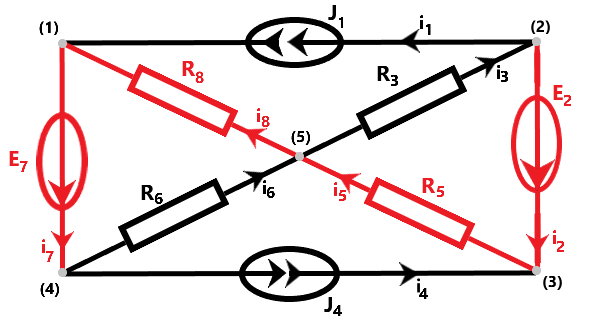
\includegraphics[width=14cm]{schema1a.png}
\caption{Circuitul cu elemente ideale de la tema 1}\label{fig1a}
\end{center}
\end{figure}


\pagebreak

Am adaugat condensatorul in paralel cu rezistorul $R_{8}$ si bobina in serie cu rezistorul $R_5$. Marimile caracteristice componentelor circuitului aveau valorile: \\

$E_2 = 5V$\\\\
$E_7 = 3V$\\\\
$J_1 = 1A$\\\\
$J_4 = 1A$\\\\
$R_3 = 1.5\Omega$\\\\
$R_5 = 1\Omega$\\\\
$R_6 = 0.5\Omega$\\\\
$R_8 = 1\Omega$\\\\


Valorile elementelor adaugate vor fi\\
$L = R_3 \cdot 100 / \pi = 150 / \pi$ mH\\
$C = R_{8} \cdot 100/ \pi = 100/ \pi$ $\mu$F\\

Frecventa surselor va fi: \\
$f = 50 Hz$, \\
iar $\omega = 2 \pi f = 100\pi$ rad/s \\

Sursele vor avea valorile:
\[
\left\{
\begin{array}{llllllll}
    $e_2(t) = 5\sqrt{2}sin(100\pi t)$\\
    $e_7(t) = 3\sqrt{2}sin(100\pi t + \frac{\pi}{4})$\\
    $j_1(t) = \sqrt{2}sin(100\pi t + \frac{\pi}{2})$\\
    $j_{4}(t) = \sqrt{2}sin(100\pi t - \frac{\pi}{4})$\\
\end{array}
\right.}
\]

Circuitul in c.a. este urmatorul: \\

\begin{figure}[h!]
\begin{center} 
\hypertarget{C2}{}
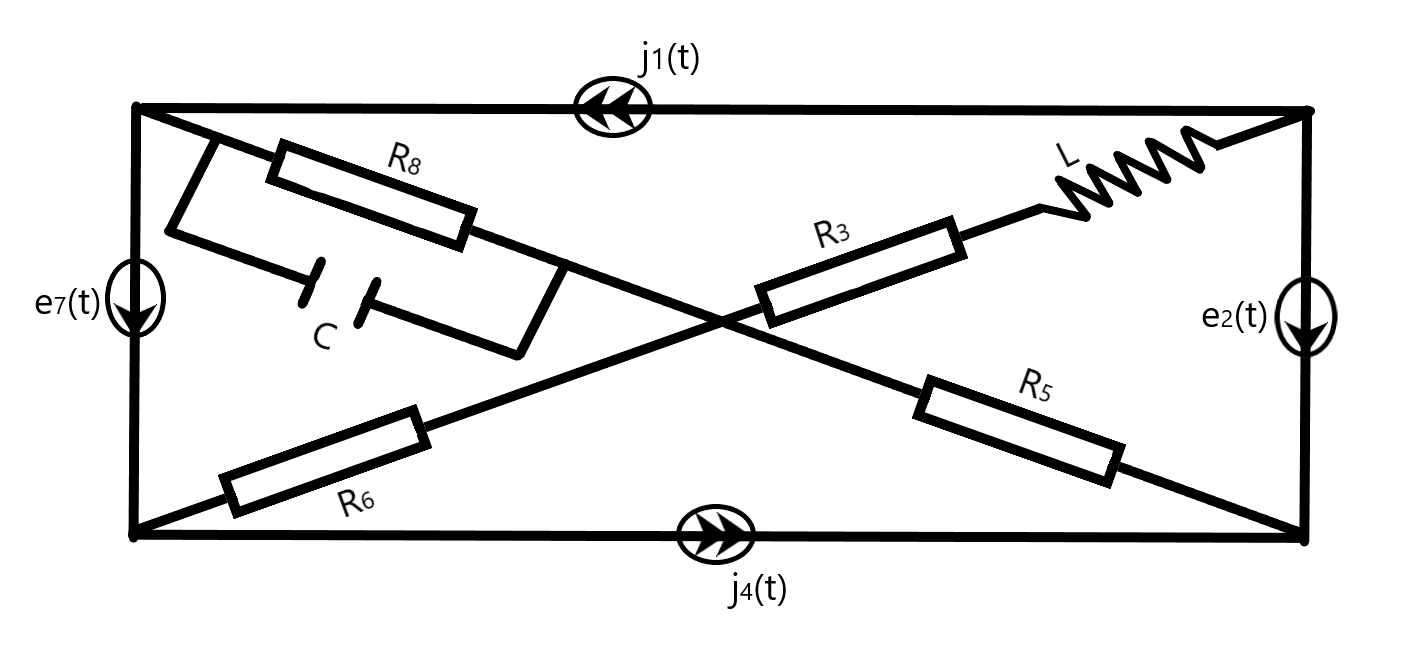
\includegraphics[width=14cm]{2.png}
\caption{Circuitul in c.a.}\label{fig1a}
\end{center}
\end{figure}


\pagebreak
In complex sursele vor avea valorile:
\[
\left\{
\begin{array}{l}
    $$\underline{E_2} = 5$$\\
    $$\underline{E_7} = 3\sqrt{2}/2 + j3\sqrt{2}/2$$\\
    $$\underline{J_8} = j$$\\
    $$\underline{J_{11}} = \sqrt{2}/2 - j\sqrt{2}/2$$\\
\end{array}
\right.}
\]

Impedantele elementelor adaugate au valorile:
\[
\left\{
\begin{array}{l}
    $$\underline{Z_{L}} = j\omega L = 15j$$\\
    $$\underline{Z_{C}} = \frac{1}{j\omega C}} = -100j$$
\end{array}
\right.}
\]


\begin{figure}[h!]
\begin{center} 
\hypertarget{C2}{}
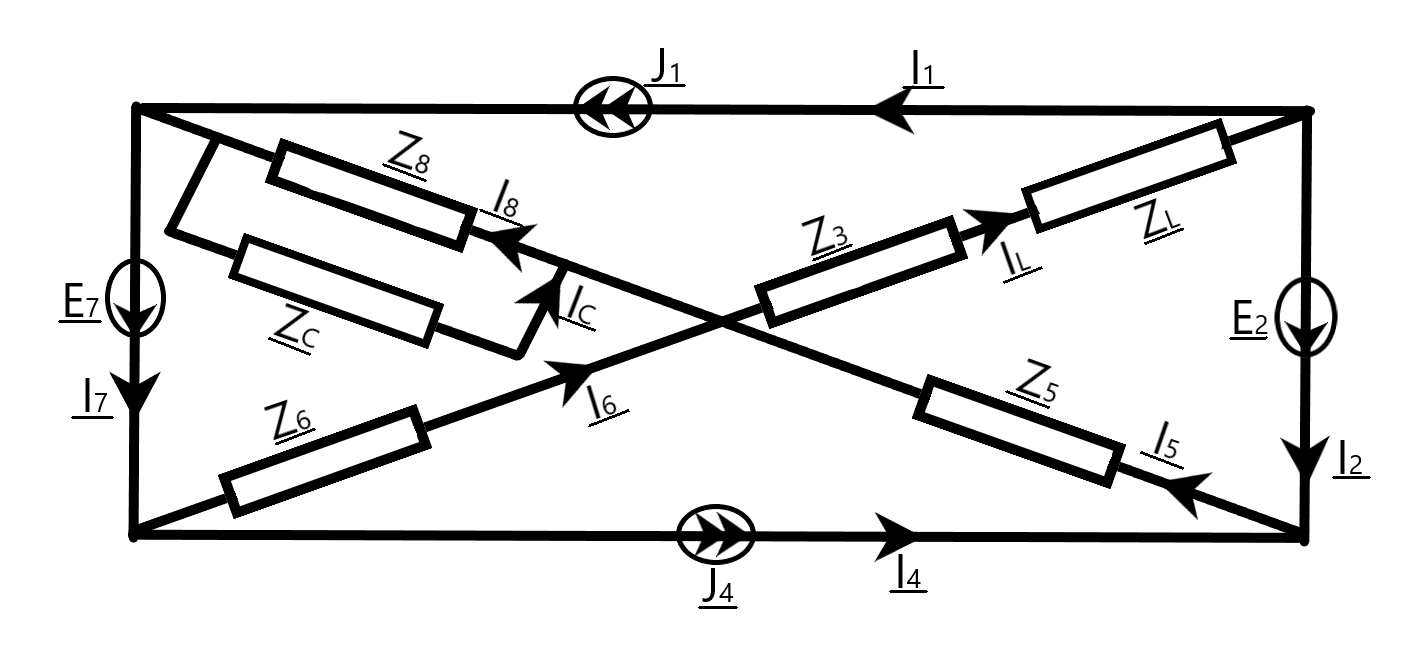
\includegraphics[width=14cm]{3.png}
\caption{Circuitul in complex}\label{fig1a}
\end{center}
\end{figure}


\pagebreak
Din prima lege Kirchhoff rezulta:\\
\[
\left\{
\begin{array}{l}
    $$\underline{I_6} - \underline{I_7} + \underline{I_4} = 0 $$\\
    $$\underline{I_4} + \underline{I_2} - \underline{I_5} = 0 $$\\
    $$\underline{I_L} - \underline{I_{2}} - \underline{I_1} = 0$$\\
    $$\underline{I_{6}} + \underline{I_{5}} + \underline{I_C} - \underline{I_{8}} - \underline{I_{L}} = 0$$\\
\end{array}
\right.}
\]\\


Aplicam apoi Kirchhoff II pe $L-N+1 = 5$ bucle:
\[
\left\{
\begin{array}{l}
    $$\underline{I_6Z_6} + \underline{I_8Z_8} = \underline{E_7}$$\\
    $$\underline{I_5Z_5} - \underline{I_6Z_6} - \underline{U_4} = 0 $$\\
    $$\underline{I_5Z_5} + \underline{I_L(Z_3 + Z_L)} = \underline{E_2}$$\\
    $$\underline{I_8Z_8} - \underline{I_L(Z_3 + Z_L)} + \underline{U_1} = 0 $ \\
    $$\underline{I_8Z_8} + \underline{I_CZ_C} = 0 $$\\
\end{array}
\right.}
\]\\


Inlocuind valorile cunoscute rezulta urmatorul sistem: \\
\[
\left\{
\begin{array}{l}
    $$\underline{I_6} - \underline{I_7} = -\sqrt{2}/2 + j\sqrt{2}/2$$\\
    $$\underline{I_2} - \underline{I_5} = -\sqrt{2}/2 + j\sqrt{2}/2$$\\
    $$-\underline{I_2} + \underline{I_L} = j $$\\
    $$\underline{I_5} + \underline{I_6} - \underline{I_8} + \underline{I_C} = 0 $$\\
    $$0.5\underline{I_6}  + \underline{I_8} = 3\sqrt{2}/2 + 3j\sqrt{2}/2$$\\
    $$\underline{I_{5}} - 0.5\underline{I_6} - \underline{U_4}  = 0 $$\\
    $$\underline{I8} - 100j\underline{I_C} = 0$$\\
    $$\underline{I_{8}} - (1.5 +15j) \underline{I_L} + \underline{U_1} = 0$$\\
\end{array}
\right.}
\]\\

Am rezolvat sistemul folosind utilitarul Matlab. In ecuatia Ax=b, A este matricea coeficientilor, x este vectorul coloana al necunoscutelor, iar b este vectorul termenilor liberi: \\
\[
    \begin{pmatrix}
    0 & 0 & 1 & -1 & 0 & 0 & 0 & 0 & 0\\
    1 & -1 & 0 & 0 & 0 & 0 & 0 & 0 & 0\\
    -1 & 0 & 0 & 0 & 0 & 1 & 0 & 0 & 0\\
    0 & 1 & 1 & 0 & -1 & -1 & 1 & 0 & 0\\
    0 & 0 & 0.5 & 0 & 1 & 0 & 0 & 0 & 0\\
    0 & 1 & -0.5 & 0 & 0 & 0 & 0 & 0 & -1\\
    0 & 1 & 0 & 0 & 0 & (1.5+15j) & 0 & 0 & \\
    0 & 0 & 0 & 0 & 1 & 0 & -100j & 0 & 0\\
    0 & 0 & 0 & 0 & 1 & (-1.5-15j) & 0 & 1 & 0
    \end{pmatrix}
    \begin{pmatrix}
    $$\underline{I_2}$$\\
    $$\underline{I_5}$$\\
    $$\underline{I_6}$$\\
    $$\underline{I_7}$$\\
    $$\underline{I_8}$$\\
    $$\underline{I_L}$$\\
    $$\underline{I_C}$$\\
    $$\underline{U_1}$$\\
    $$\underline{U_4}$$
    \end{pmatrix}=
    \begin{pmatrix}
    $-\sqrt{2}/2 + j \sqrt{2}/2$\\
    $-\sqrt{2}/2 + j \sqrt{2}/2$\\
    $j$\\
    $0$\\
    $3\sqrt{2}/2 + 3j\sqrt{2}/2$\\
    $0$\\
    $5$\\
    $0$\\
    $0$
    \end{pmatrix}
\]\\
\pagebreak

Solutia acestui sistem este urmatoarea:\\
\begin{figure}[h!]
\begin{center} 
\hypertarget{C2}{}
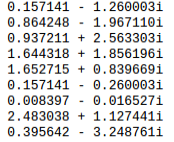
\includegraphics[width=6cm]{solutii.PNG}
\caption{Solutia sistemului}\label{fig1a}
\end{center}
\end{figure}
\subsection{Calcularea bilantului de puteri}
In urma calculelor am obtinut urmatoarele puteri\\

$S_{gen} = 11.9158 +  1.3501i$\\

$S_{cons} = 11.9158 +  1.3501i$\\

Asadar, bilantul de puteri se verifica, calculele sunt corecte.


\subsection{Reprezentarea grafica a intensitatii prin bobina}

Pentru a realiza variatia in timp a intensitatii prin bobina am folosit functiile "angle" si "abs" din Matlab. Am considerat 1000 de puncte in intervalul [0,0.1]. Forma in complex a intensitatii este: \\

$$\underline{I_L} = 0.157141 - 0.260003i$$\\

$$i_L(t) = abs(\underline{I_L}) \cdot \sqrt{2} \cdot sin(100\pi t + angle(\underline{I_L})$$\\
\begin{figure}[h!]
\begin{center} 
\hypertarget{C2}{}
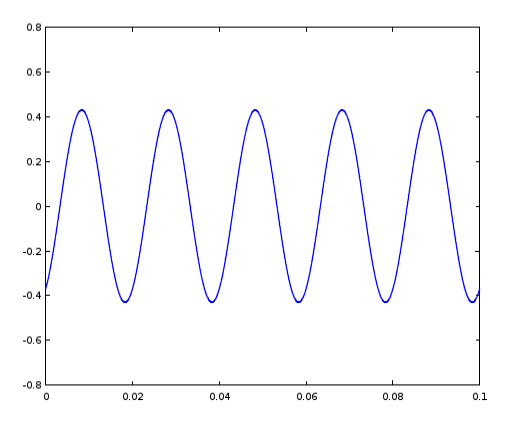
\includegraphics[width=10cm]{ex1plot.PNG}
\caption{Graficul intensitatii prin bobina}\label{fig1a}
\end{center}
\end{figure}

Graficul este valid deoarece valoarea maxima a intensitatii obtinuta prin calcule este aceeasi cu cea reprezentata grafic:
$$abs(\underline{I_L}) \cdot \sqrt{2} = 0.42964$$


\section{Exercitiul 2}
\subsection{Valorile initiale ale elementelor adaugate}

Pentru rezolvarea acestui exercitiu am lasat bobina si condensatorul pe aceleasi laturi folosite la primul exercitiu.

Valorile initiale ale elementelor adaugate sunt cele obtinute la tema 1,adica, $i_L(0_-) = 2A$, iar $u_C(0_-) = 2V$.

\subsection{Rezolvarea circuitului in regim tranzitoriu}

La momentul $t = 0$ am eliminat latura cu sursa $E_2$. \\

Valorile elementelor in regim tranzitoriu sunt urmatoarele:\\\\
$e_7(s) = 3/s$\\
$j_1(s) = 1/s$\\
$j_4(s) = 1/s$\\
$sL(0_-) = \frac{0.15s}{\pi}$\\
$Li_L(0_-) = \frac{0.3}{\pi}$\\
$u_C(0_-)/s = \frac{2}{s}$\\
$\frac{1}{sC} = \frac{10^4\pi}{s}$\\
\\

Dupa trecerea elementelor circuitului in regim tranzitoriu se obtine urmatorul circuit:\\

\begin{figure}[h!]
\begin{center} 
\hypertarget{C2}{}
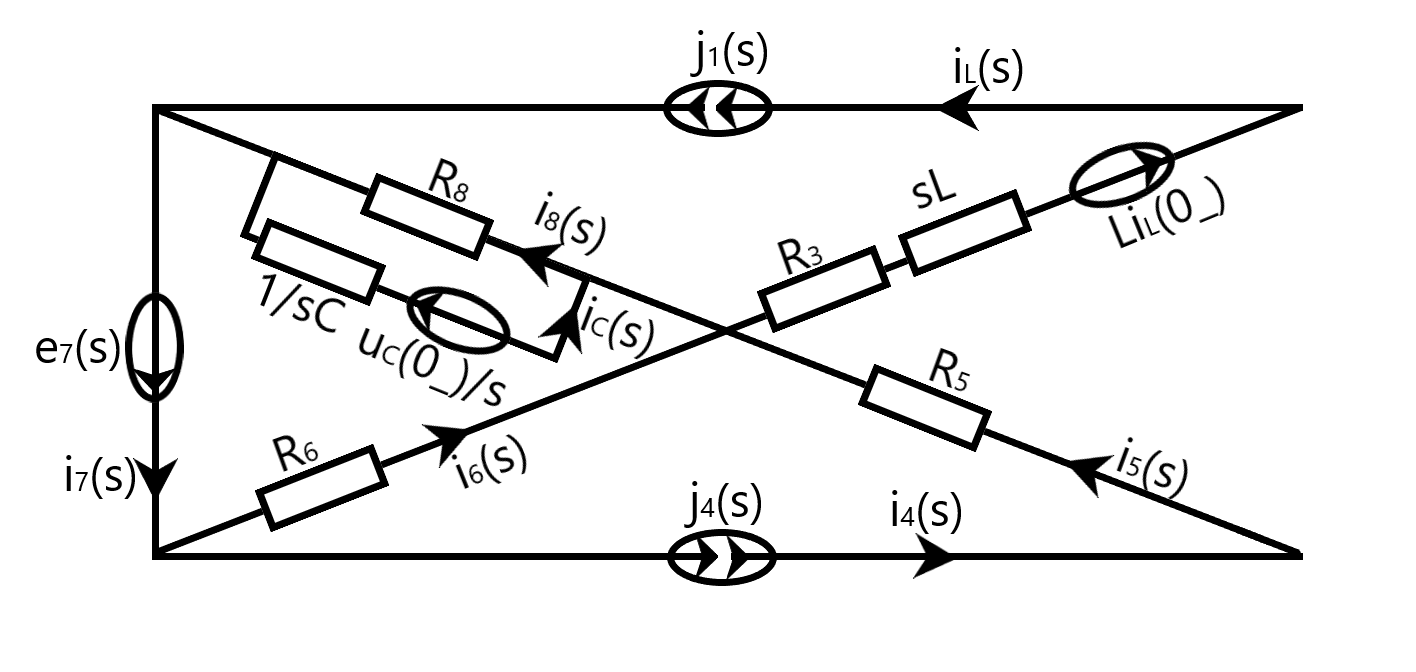
\includegraphics[width=14cm]{4.png}
\caption{Circuitul cu elemente ideale de la tema 1}\label{fig1a}
\end{center}
\end{figure}


Aplicam prima lege a lui Kirchhoff pe $N-1$ noduri: \\
\[
\left\{
\begin{array}{l}
    $$i_7(s) - i_6(s) - i_4(s) = 0 $$\\
    $$i_6(s) + i_c(s) + i_4(s) - i_8(s) - i_L(s) = 0$$\\
\end{array}
\right.}
\]\\

In continuare am aplicat a doua lege a lui Kirchhoff pe $L-N+1 = 4$ bucle:\\
\[
\left\{
\begin{array}{l}
    $$i_L(s)(R_3 + s_L) - u_1(s) = Li_L(0_)$$\\
    $$R_{8}i_8(s) + i_C(s)\frac{1}{sC} = \frac{-u_C(0_-)}{s}$$\\
    $$R_6i_6(s) + i_8(s)R_8 = e_7(s)$$\\
    $$i_6(s)R_6 - i_4(s)R_5 + u_4(s) = 0$$
\end{array}
\right.}
\]\\
Cum bobina este in serie cu o sursa de curent ($J_1$), i_L(s) = j_1(s) = \frac{1}{s}\\

Inlocuind valorile cunoscute obtinem urmatorul sistem: \\
\[
\left\{
\begin{array}{l}
    $$-i_6(s) + i_7(s) = \frac{1}{s}$$\\
    $$i_6(s) - i_8(s) + i_C(s) = 0 $$\\
    $$0.5i_6(s) + u_4(s) = \frac{1}{s}$$\\
    $$u_{1}(s) = \frac{1.5}{s} -\frac{0.15}{\pi} $$\\
    $$i_8(s) + i_{c}(s) \cdot \frac{10^4 \pi}{s} = -\frac{2}{s}$$\\
    $$0.5i_{6}(s) + i_8(s) = \frac{3}{s}$$\\
    \end{array}
\right.}
\]\\

Acesta este un sistem de forma $Ax = b$ pe care l-am rezolvat in Matlab, obtinand $u_C(s) = \frac{-2s + 188400}{s(s+94200)}$.\\
\begin{figure}[h!]
\begin{center} 
\hypertarget{C2}{}
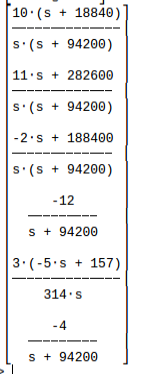
\includegraphics[width=3.2 cm]{ex2res.PNG}
\caption{Solutia sistemului}\label{fig1a}
\end{center}
\end{figure}


\pagebreak
\subsection{Trecerea in timp a rezultatelor obtinute}

Am obtinut $i_L(s) = \frac{1}{s}$.
La aplicarea transformatei Laplace inversa se obtine $i_L(t) = 1$.\\

Verific conditiile initiale:\\
$$\lim_{s\to\infty} s*i_L(s) = s \cdot \frac{1}{s} = \lim_{t\to 0} i_L(t) = 1$$\\

Verific conditiile finale:\\
$$\lim_{s\to 0} s*i_L(s) = s \cdot \frac{1}{s} = \lim_{t\to\infty} i_L(t) = 1$$\\\\

Intrucat cele doua valori sunt egale putem trage concluzia ca sunt verificate conditiile initiale.
\pagebreak
\subsection{Graficul in timp}
\begin{figure}[h!]
\begin{center} 
\hypertarget{C2}{}
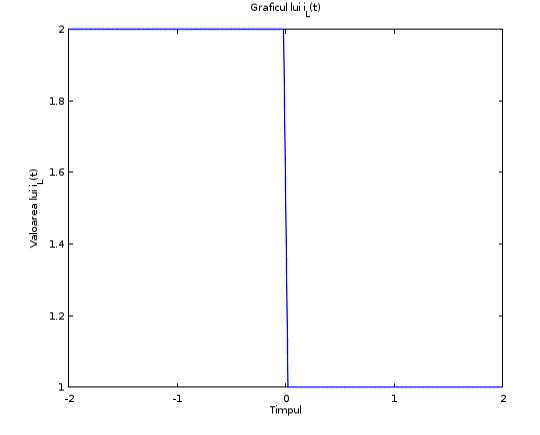
\includegraphics[width=14cm]{ex2plot.PNG}
\caption{Graficul in timp }\label{fig1a}
\end{center}
\end{figure}
\pagebreak


\section{Exercitiul 3}
\subsection{Aflarea lui D(r)}
Am considerat distributia de sarcina de forma:\\\\
$\rho(r,\theta,\phi) =
\[
\left\{
\begin{array}{l}
    2 + r^2,  r\epsilon [0,a]\\
    0, r>a
\end{array}
\right.}
\]\\$
\\

$\int_{\Sigma} D dA = \int_{D_{\Sigma}} \rho dV$\\
$q = \int\int\int \rho dV$\\

Se disting doua cazuri:\\
Cazul I: $r\geq a$\\\\
$q = \int_{0}^{a} (2+r^2)\cdot 4\pi r^2dr$ \\
$q = 4\pi \cdot (2\frac{r^3}{3} + \frac{r^5}{5})|_{0}^{a}$\\
$q = 4\pi \cdot (\frac{3a^4}{3} + \frac{a^5}{5})$\\
$\Rightarrow D(r) = \frac{1}{r^2} \cdot (\frac{a^3}{3} + \frac{a^5}{5})$\\\\


Cazul II: $0 < r < a$:\\\\
$q = \int_{0}^{r} (2 + r^2) \cdot 4\pi r^2 dr$\\
$q = 4\pi \cdot (\frac{2r^3}{3} + \frac{r^5}{5})\\
$\Rightarrow D(r) = \frac{q}{4\pi r^2} = \frac{2r}{3} + \frac{r^3}{5}$\\\\

Deci in final inductia electrica D(r) este: \\
$D(r) =
\[
\left\{
\begin{array}{l}
    \frac{1}{r^2} \cdot (\frac{a^3}{3} + \frac{a^5}{5}, r>a\\
    \frac{2r}{3} + \frac{r^3}{5}, 0<r<a
\end{array}
\right.}
\]\\$
\\
\pagebreak

\subsection{Reprezentarea grafica a spectrului lui D(r)}
In reprezentarea spectrului si echivalorilor lui D am considerat $a = 4$
\[
  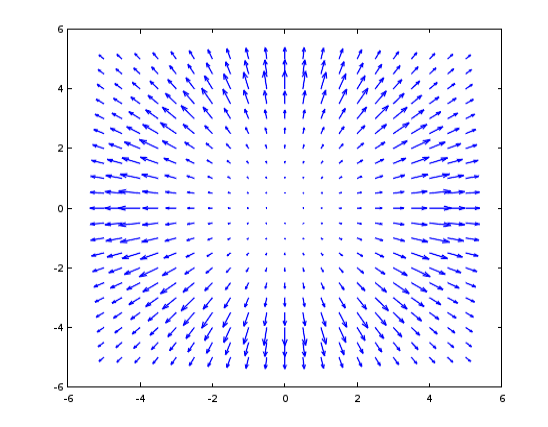
\includegraphics[width=350]{ex3b.PNG}
\]\\
\pagebreak

\subsection{Reprezentarea grafica a echivalorilor}
\[
  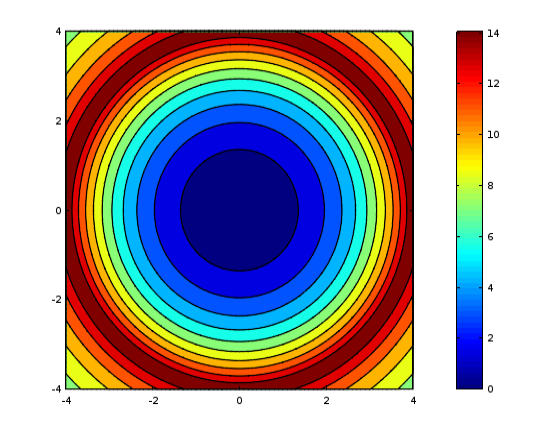
\includegraphics[width=350]{ex3c.PNG}
\]\\
\pagebreak
\section{Bibliografie}
1.  cs.curs.pub.ro - prof. Gabriela Ciuprina\\

2. sharelatex.com\\

3. http://web.ift.uib.no/Teori/KURS/WRK/TeX/symALL.html
\end{document}